%!TEX encoding = UTF-8 Unicode
\chapter{概述}
要分析Android恶意代码,首先要对Android系统的一些基本知识有所了解,例如APK文件格式、应用软件开发方式和编译过程,还需要对系统内部结构有所认识,包括DEX文件结构、Dalvik指令集、Android系统结构等。可惜的是,这些知识散落在Android文档和书籍之中,并没有被专门地整理和介绍。本章对这些知识单独做介绍,但DEX文件结构和Dalvik指令集等过于重要,将单独作为后面的一章。

除了本章的内容,我们建议读者多阅读Android的开发文档和源码(尤其是源码中的文档)。此外,还有几本关于Android系统原理分析的书\cite{android_jishuneimu, android_shenrulijie, android_neihepouxi},也值得一看。
\section{系统结构}
Android系统的组成结构如图\ref{Fig:system-architecture}所示,主要分为四层,自底向上分别是Linux内核与驱动、系统库和虚拟机、应用程序框架、应用程序。
\begin{figure}[htbp]
  \centering
  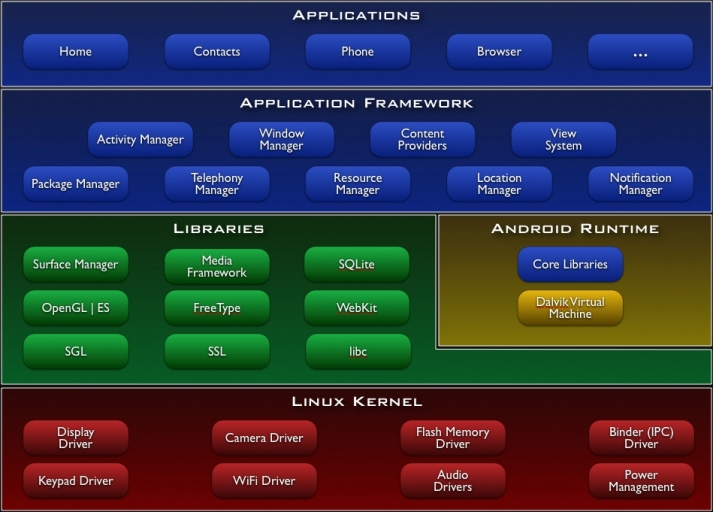
\includegraphics[width=14cm]{image/system-architecture.jpg}
  \caption{Android系统结构}
  \label{Fig:system-architecture}
\end{figure}

\subsection{Linux内核与驱动}
Android完整地使用Linux内核,获得内存管理、进程管理、文件管理、用户管理、进程间通信等能力。

为了控制手机的一些特有硬件,例如摄像头、触控屏、蓝牙等,这一层还包含这些硬件设备在Linux上的驱动程序。

这一层向上提供的接口是硬件抽象层(HAL),Android规定了HAL的接口规范。手机厂商可以针对不同的设备分别开发驱动,并以统一的接口为高层提供服务,也就是所谓的Android系统移植。

\subsection{系统库和虚拟机}
Android系统库包括大量被上层复用的基本功能,例如标准C库libc浏览器引擎Webkit、数据库管理系统SQLite、图像处理OpenGL等。

Android使用一种称之为Dalvik的虚拟机。它非常类似于Java虚拟机JVM,但并不是真正的JVM。事实上,JVM虽然有垃圾回收等机制,但并非为移动设备而设计,在运行速度、资源占用等方面难以满足移动终端硬件的苛刻眼球。因此,Android实现了Dalvik。从实现方式上看,两者的最大区别在于Dalvik是基于寄存器的结构,而JVM是基于栈的结构。

\subsection{应用程序框架}
这一层体现了Android对移动设备应用程序的理解。它隐藏了系统中进程、内存管理等概念;针对不同应用需求抽象出活动(activity)、服务(service)、内容提供者(content provider)、广播接收器(broadcast receiver)的概念;提供了窗口管理、通话管理、软件包管理、资源管理、地理位置管理等常用的功能。

这一层向上提供了Java形式的Android应用程序开发的框架与接口。

\subsection{应用程序}
在最高层,软件开发者通过Java语言和下层框架接口,在Android平台开发各类特色应用。

Android随系统附带了一些应用程序,比如通话、通讯录、Web浏览器、软件列表等基本功能。这也意味着,用户所见到的手机界面和功能,实际上都是这一层的一个或多个应用程序。这种设计思想使得用户的所有操作都通过规定的框架和接口调用底层,保证了系统的稳定性和安全性。

\section{Android软件开发}
除了上面提到过的系统移植,Android相关的开发可以简单地分为系统开发和应用程序开发。两者都不涉及与硬件的直接交互。

\subsection{系统级开发}
系统开发面向第二层,即系统库之中。开发者使用C或C++语言,调用Linux内核、Android系统库提供的接口,增加系统的功能。这些新增的功能以库文件形式增加到系统中,通过JNI\footnote{Java Native Interface,是Java标准的一部分,允许Java代码与其他语言写的代码进行交互。}供顶层的普通应用程序调用。

Android提供了NDK(Native Development Kit)工具支持这种开发。开发者可以使用NDK将C/C++代码编译为.so动态链接库文件,并打包到.apk安装包中。程序在运行时将.so文件解压到本地目录并加载,供自身调用。这样,开发者就不需要编译集成整个系统就能做到系统开发了。

除了被顶层程序作为功能模块调用,从NDK Revision5开始,可以完全用C/C++编写一个完整的应用程序。但我们并不推荐这种开发方法,因为GUI组件的生命周期管理等工作需要自行编码实现,工作量大而稳定性差。NDK开发的优点在于,它可以利用一些底层的库函数,在图像处理等高运算量工作上运行速度会明显快于Java开发的程序(后者运行于Dalvik虚拟机之中)。此外,它还是一种极为重要的软件保护机制,我们会在后续章节再次讨论。

值得我们注意的是,传统的个人计算机大都运行在x86架构的CPU之上,因此可执行文件都是基于x86的二进制码。但Android手机一般采用ARM架构的CPU,因此其内核、系统库等可执行文件都是基于ARM的二进制码。因此,系统开发中的编译不能用PC上的gcc等工具。实际上,这类开发与嵌入式开发一样,需要用到所谓的交叉编译技术,即使用特殊的编译器,其自身是x86格式,而生成的目标文件是ARM格式。NDK提供了包括调试工具在内的完整工具链。

\subsection{应用程序开发}
Android上应用程序的开发使用Java语言。有两种开发环境可以选择:
\begin{itemize}
	\item 图形界面环境,使用Eclipse和Android ADT
	\item 命令行环境,使用Apache Ant
\end{itemize}
开发环境的建立可以参考SDK文档或者任何一本介绍Android开发的书籍。

Android为封装了多种GUI控件,以Java类的方式提供给开发者。例如,文本框TextView、列表ListView、按钮Button、菜单Menu、图片ImageView、状态栏提示Notification等。开发者直接实例化这些类,并设置属性和动作,就可以开发丰富的GUI程序了。此外,还可以调用SQLite创建和访问数据库、调用Socket访问网络、调用OpenGL开发游戏等。

\subsection{编译流程}
一个典型的Android工程包括下列文件和文件夹:
\begin{itemize}
	\item AndroidManifest.xml:主配置文件,描述了软件名、系统版本、运行所需权限、基本组件、Intent-filter信息等
	\item assets/:包含程序需要使用的其他文件
	\item bin/:包括最后生成的.apk安装包
	\item default.properties:Eclipse使用的项目配置文件
	\item build.properties:Ant使用的项目配置文件
	\item jni/:包括NDK开发的C/C++源码,以及Makefile文件
	\item libs/:包括NDK编译出来的.so文件
	\item res/drawable/:图标、图片资源
	\item res/layout/:布局资源,由XML语言描述
	\item src/:包括Java源码文件,按package的结构组织
\end{itemize}

编译流程如图\ref{Fig:compilation}所示。
\begin{figure}[htb]
  \centering
  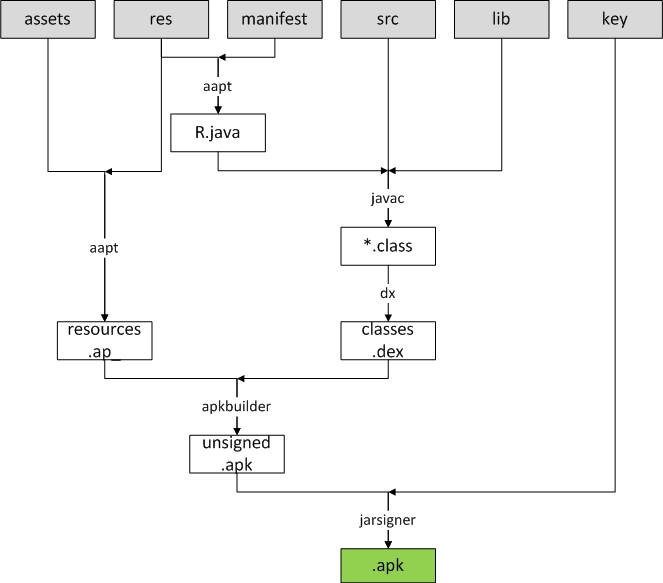
\includegraphics[width=14cm]{image/compilation.jpg}
  \caption{Android应用程序编译流程}
  \label{Fig:compilation}
\end{figure}

具体而言:
\begin{enumerate}
	\item 使用SDK中的aapt工具,从资源文件夹res/中,生成源码R.java,其中包含了一个名为R的Java类,该类对所有需要引用的资源建立数字索引,从而将src/下的Java源码与各类资源关联;
	\item 使用Java SDK中的javac工具,将所有Java源码编译为对应的.class文件;
	\item 使用SDK中的dx.bat,将所有.class文件转换为一个classes.dex文件。前面我们提到,Android使用了自己定义并实现的Dalvik虚拟机,它的可执行文件即.dex格式。
	\item 使用aapt,将res/下的资源文件打包为resource.ap\_;
	\item 使用SDK中的apkbuilder.bat,将配置文件、资源包、classes.dex等,打包为未签名的.apk安装包;
	\item 使用SDK中的jarsigner工具,对上述安装包签名,最终得到可以安装的已签名.apk安装包
\end{enumerate}

\section{APK文件格式}
Android系统使用的安装包文件后缀名为.apk。实际上它是标准的ZIP格式文件,可以使用7-zip等压缩软件、zlib等函数库进行处理
\footnote{ZIP格式的详细介绍,参考\url{http://en.wikipedia.org/wiki/ZIP\_(file\_format)}。}。

一个.apk文件解压缩后,通常包括如下文件或文件夹:
\begin{itemize}
	\item[-] AndroidManifest.xml:项目配置文件,但不是明文的XML文件,直接打开无法阅读
	\item[-] classes.dex:所有的Java类文件被打包并转换为这个文件,它是Dalvik虚拟机上的可执行二进制文件,Android系统在运行时将其动态优化为.dey文件并投入一个Dalvik虚拟机实例中运行。
	\item[-] resources.arsc:资源文件打包而成,字符串值(源码中res/value/Strings.xml)就在其中
	\item[-] res/:资源文件夹,其中包括布局文件夹layout、图标图片文件夹drawable、原始文件文件夹raw(该目录下任何文件都会原封不动地存储到设备上)等
	\item[-] META-INF/:数字签名文件夹
	\item[-] lib/:包含NDK开发中使用的动态链接库文件(ARM架构下ELF格式.so文件),有的软件没有这个文件夹
	\item[-] assets/:原始文件文件夹,其中的文件不会被压缩,也不能想res/目录下的资源文件一样通过R类引用,有的软件没有这个文件夹
\end{itemize}

其中,数字签名文件夹META-INF/包含下列文件:
\begin{itemize}
	\item[-] CERT.SF:生成每个文件相对的密钥
	\item[-] MANIFEST.MF:数字签名信息
	\item[-] xxx.SF:这是 JAR 文件的签名文件,xxx标识了签名者
	\item[-] xxx.DSA:对输出文件的签名和公钥
\end{itemize}

